\documentclass[10pt]{article}
\usepackage[a4paper,margin=18mm]{geometry}
\usepackage{amsmath,amssymb,booktabs,graphicx,xcolor,hyperref}
\hypersetup{colorlinks=true,urlcolor=blue}
\setlength{\parindent}{0pt}
\setlength{\parskip}{5pt}
\newcommand{\softO}{\widetilde O}
\begin{document}
{\LARGE Exponent-moving ideas for Curve25519}\par
17 November 2026 \quad Analytical proposal; producer unsigned/unverified.

\textbf{Priority: an implicit six-sum join.} Seek more than $B$ checked,
privately tagged relations in total work $B^{3-\varepsilon}$ at
$B\asymp N^{1/6}$. This is a concrete missing algorithm, not a claim that it
exists. The alternative leads below seek the same structural saving.

The instance is $v^2=u^3+486662u^2+u$ over $p=2^{255}-19$, with cofactor
8 and prime subgroup order
$N=2^{252}+27742317777372353535851937790883648493$.
The original six-member circuit has 1059 variables and 1089 equations,
$a=60824497,q=213156431,k=20633$. Its current base is not silently equated
with $N^{1/6}$. No experiment, source test, solver campaign or paid job ran.

\textbf{The conditional cost contract.} With $B=N^\beta$, fixed arity $m$,
expected attempted-query cost $D$, useful returned-root probability $y$,
setup $P$, kernel $K$ and final recovery $H$, charge one cold DLP:
\[
 C=P+O(B)D/y+K+H.
\]
Use the existing controller-private coefficient protocol: retain $R>B$
rows over common columns and choose a nonzero left-kernel vector without
seeing coefficient tags. Full rank or independent rows are not required;
the actual selection/point/cost bridges still are.

If $D=\softO(B^\gamma)$,
$y\gtrsim N^{-\eta}\min(1,B^m/N)$ up to subpolynomial factors,
and the other phase exponents are $\sigma,\lambda,\delta$, then
\[
 \alpha=\max\{\sigma,\lambda,\delta,
 (1+\gamma)\beta+\max(0,1-m\beta)+\eta\}.
\]
Assuming $P+K+H=\softO(B^2)$ and $\eta=0$ gives the following
\emph{illustrative hypothetical points}, already in scaling-audit-v1:
\begin{center}
\begin{tabular}{@{}llll@{}}
\toprule
Arity & Strict query target & Example $\gamma,\beta$ & Total model exponent\\
\midrule
4 & $\gamma<1$ & $1/2,\;2/9$ & $4/9$\\
6 & $\gamma<2$ & $3/2,\;1/6$ & $5/12$\\
8 & $\gamma<3$ & $5/2,\;1/8$ & $7/16$\\
\bottomrule
\end{tabular}
\end{center}
At the six-sum example an extra yield loss $\eta=1/12$ consumes the
entire square-root margin. All failed queries, original-root lifting,
decoding and replay belong in $D$. A finite favorable fit cannot replace a
growing-family argument. These formulas are producer derivations, not a
new attack bound or signed validation.

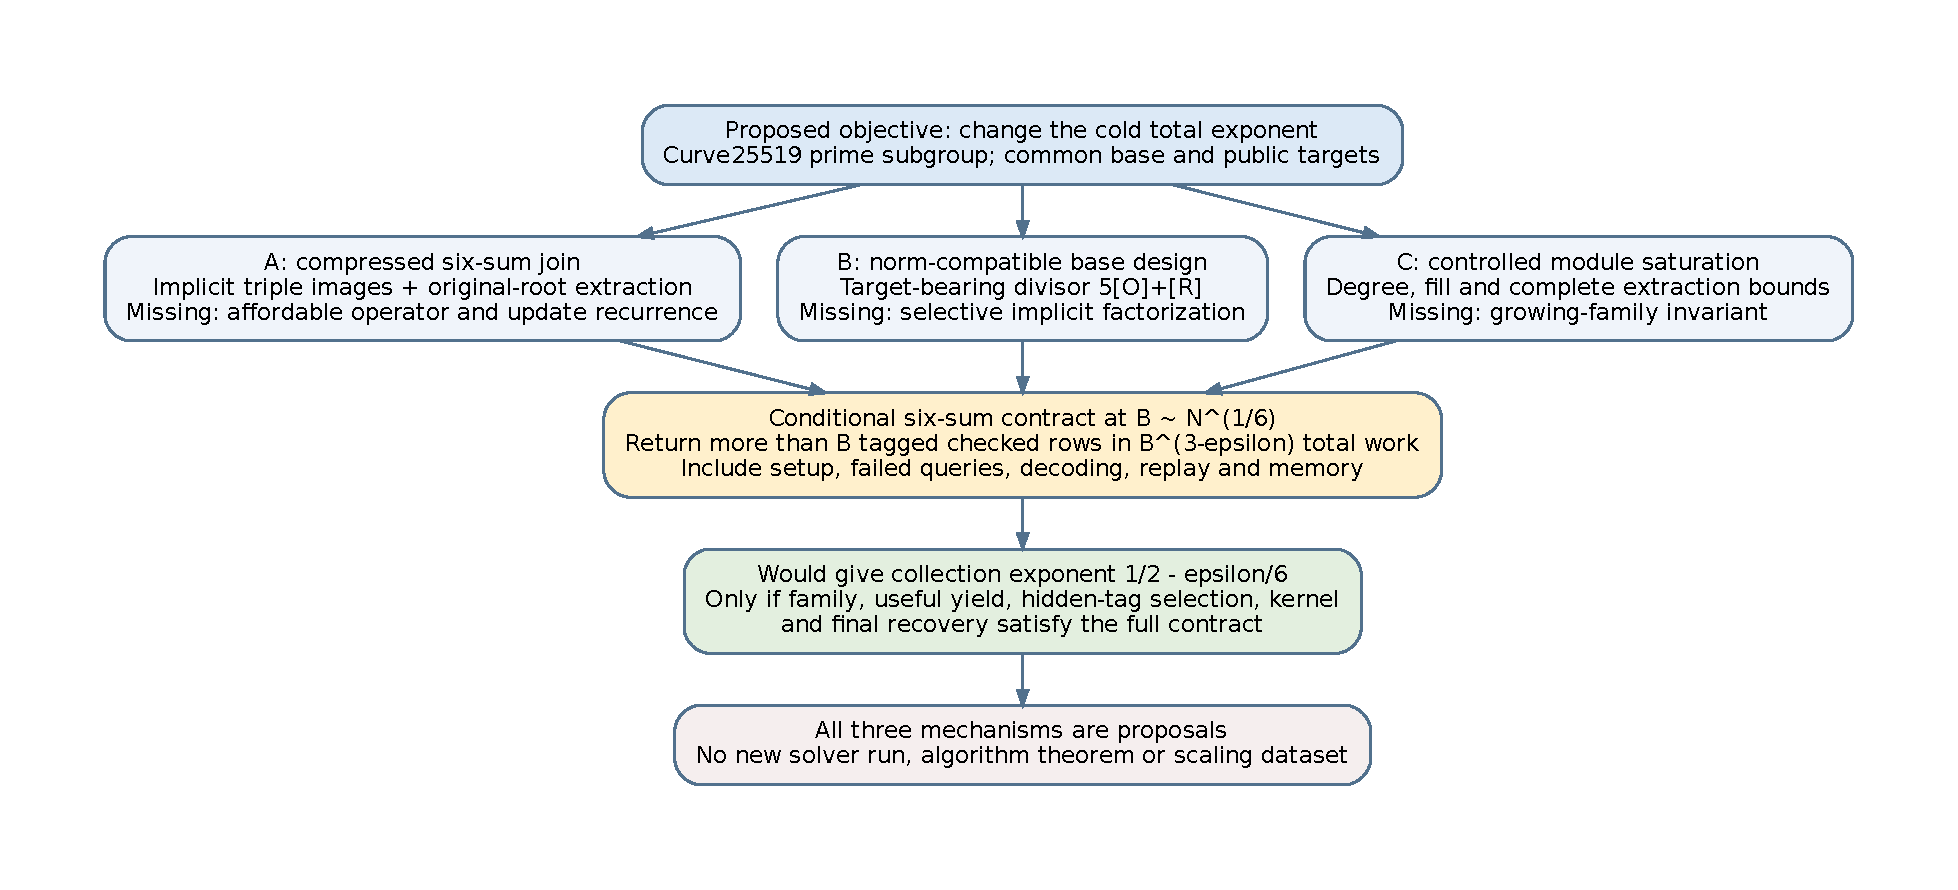
\includegraphics[width=\linewidth,height=78mm,keepaspectratio]{mechanisms.pdf}

\newpage
{\Large Three mechanism cards}\par
\textbf{A. Compressed elliptic six-sum joins --- first priority.}

For a compact base map $\Phi$, find original roots of
\[
 \Phi(z_1)+\Phi(z_2)+\Phi(z_3)
 =T-\Phi(z_4)-\Phi(z_5)-\Phi(z_6).
\]
Retain every coset/index, chart, ordinate, sign, cofactor and distinct-column
guard. Torus multiplication is not elliptic addition. Explore quotient-ring
modular composition, structured resultants and translation operators with
low displacement complexity. Require an exact existence/counting operator
stable under prefix restrictions, followed by original-witness extraction.
Field-count cancellation is not emptiness.

\emph{Next deliverable:} public-coordinate operator entries, compressed
representation, update/extraction recurrence and a bound below $B^3$ for
more than $B$ accepted tagged rows. This would give collection exponent
$1/2-\varepsilon/6$ only if all remaining phases and useful yield fit.

\emph{Scoped rejection:} triple enumeration, cubic coefficient expansion,
unknown logarithm labels or cubic extraction defeats that instantiation at
this model point. A rational annihilator vanishing on $s$ distinct points
has pole degree at least $s$; if triple support is $\Theta(B^3)$, ordinary
dense storage does not provide the saving. Compact high-degree structures
remain open. Full matrix rank alone does not rule out fast multiplication.

\textbf{B. Norm-compatible base and relation design.}

Design membership jointly with constrained norm factorization, using
\[
 \operatorname{Norm}(A(u)+vB(u))
 =A(u)^2-(u^3+486662u^2+u)B(u)^2.
\]
For a public target $R$, a function with full pole divisor $5[O]+[R]$
and six base-supported rational zeros gives a six-sum to $R$. Riemann--Roch
gives a six-dimensional function space, not the desired function. Restore
denominators, multiplicities and signed orientations.

\emph{Next deliverable:} one compact norm/base identity, an exact lift to the
signed original relation, selective factorization and a useful-target bound.
Require the same full cost threshold as A. Blind sampling, planted zeros,
or homogeneous relations without a DLP bridge do not meet it. Under a uniform
divisor heuristic blind success is about $(B/p)^6$; this warning is not a
proved algorithmic lower bound.

\textbf{C. A family-wide degree and extraction invariant.}

Seek a saturation schedule with bounded monomials, fill and complete root
extraction on both consistent and inconsistent targets. Affine quotienting
is only a support test. A dense $M^\omega$ routine must fit below $B^2$ for
the six-sum per-query target, with all other costs included. Bounded solving
degree with logarithmically many variables would be an ingredient only if
the actual encoding and extraction justify it.

\emph{Next deliverable:} an exact invariant and complete extraction/cost
argument. First fall degree is insufficient. The old constant-row-space
audit found no new input-only combinations on the fixed original input
(PCC-20261117-f9b20c, unsigned/unverified); it is not an ideal or family
exclusion. A violating input rejects a universal lemma; a cap parks a run.

\newpage
{\Large What to avoid, and what to do next}\par
\textbf{Secondary arithmetic lead.} A small-height base might use the
pseudo-Mersenne modulus and small curve coefficients. Before a lattice run,
give the exact integer lift, carry variables, height/determinant bounds and
independent root-isolating polynomials. Full-size target coefficients and
multivariate modular equations do not inherit classical univariate modular
or bivariate integer bounds. Review existing joint-smallroot-native work
before implementation; it was located, not reviewed in depth here.

\textbf{Wagner is not a coordinate-hash shortcut.} The original paper also
handles integer modular sums through interval joins; prime order alone does
not reject all generalized-birthday methods. Elliptic coordinate bits are
not accessible scalar intervals. An exact homomorphism from $C_N$ to a group
without $N$-torsion is trivial. Approximate filters still need selective,
cheap compatible joins with retained roots. Generic-operation lower bounds
do not exclude a genuine representation-specific mechanism.

\textbf{Representation alone does not supply a rate.} A fixed-degree map,
bounded automorphism fold, shorter equation or more cores needs an actual
cost or degree argument before it supports an exponent claim. A twist needs
recoverable subgroup transport. At $B=N^{1/6}$, the current enumerating
reference already spends $B^3=N^{1/2}$ on setup; increasing caps does not
meet A. All reuse within one DLP is charged to that DLP.

\textbf{Order of work.} First derive A's operator and recurrence. Keep B as a
distinct algebraic construction task. Use C's affine quotient only against
a stated invariant. Before escalation require the actual base cardinality,
an admissible growing family, useful yield, hidden-tag selection, common
columns, kernel/recovery costs and memory. Rust/native implementation and
separate qualification follow only after a concrete algorithm is specified.
No new experiment is admitted or scheduled by this document.

\textbf{Route outcomes.} Keep ROUTE\_CRITERIA\_V3.md unchanged: exact
counterexample, proved scoped exclusion, rejected finite quantitative
promise, parked implementation, invalid experiment or open. No failed
representation rejects all index calculus. T2 separately retains its
six-size/24-order-bit/held-out and independent validation requirements.

\textbf{Primary sources read.} Full passages and bounded repository review
are in SOURCES.md. PKM2016 sections 3--5 already ask for dedicated generalized
root finding; Kosters--Yeo separates first fall from solving complexity;
Diem2011 uses genuine subfields; Huang et al.2020 requires a characteristic-
power structure not instantiated over this prime field. Bhargava et al.2022
takes a coefficient vector, not an implicit root-finding input. Wagner's
author long version was downloaded as PostScript and read after conversion.
Snowden's Math679 lecture supplies divisor/Riemann--Roch facts. Coppersmith's
author abstract was read; the full 1997 PDF fetch failed and no exact lattice
threshold is borrowed from it.

\textbf{Existing work and novelty.} The repository already has tensor
counting-to-search, compositional bases, binary quasi-subfield searches,
partial sparse elimination and fixed row-space audits. Their missing cost
bridges are not new algorithms. This report nominates targets and derives
conditional thresholds; it makes no novelty claim. KB is unavailable (no MCP;
wrapper exits 127). Conductor is unconfigured (127), documented warning-only
fallback. No reservation or delegation is claimed.

\textbf{Publication scope.} The Markdown contains the full envelope derivation,
including its parameter limits. The diagram is editable and proposal-labeled.
No measured performance value, leaderboard row or established map edge was
added; canonical scoreboards stay unchanged. No existing frozen input,
criteria, source or raw result was edited. All mathematical assertions here
remain producer unsigned/unverified pending independent review.
\end{document}
